\pdfoutput=1 % for arXiv to use pdflatex
\documentclass[12pt]{article}

%% The graphicx package provides the includegraphics command.
\usepackage{graphicx}
%% The amssymb package provides various useful mathematical symbols
\usepackage{amsmath}
\usepackage{amssymb}
%% The lineno packages adds line numbers. Start line numbering with
%% \begin{linenumbers}, end it with \end{linenumbers}. Or switch it on
%% for the whole article with \linenumbers after \end{frontmatter}.
\usepackage{lineno}
\usepackage{url}
\usepackage{xspace,multicol}
\usepackage{siunitx}
\usepackage{subcaption}
\usepackage{color, colortbl}
%\usepackage{units}
\usepackage{ragged2e}
\usepackage{array}
\usepackage{tabularx}
\usepackage{authblk}
\usepackage{heppennames}
\usepackage{feynmp}
\usepackage{libertine}
% \usepackage[libertine]{newtxmath}
\usepackage{textgreek}
\DeclareGraphicsRule{*}{mps}{*}{}

\newcommand{\guineapig}{GuineaPig\xspace}
\newcommand{\sid}{SiD\xspace}
\newcommand{\electron}{e\textsuperscript{-}\xspace}
\newcommand{\positron}{e\textsuperscript{+}\xspace}
\newcommand{\micron}{\ensuremath{\murm\mathrm{m}\xspace}}

\newcommand{\murm}{%
  \ifmmode
    \mathchoice
        {\hbox{\normalsize\textmu}}
        {\hbox{\normalsize\textmu}}
        {\hbox{\scriptsize\textmu}}
        {\hbox{\tiny\textmu}}%
  \else
    \textmu
  \fi
}


\usepackage{fixltx2e}


\begin{document}

%% Title, authors and addresses

\title{Impact of the new ILC250 Parameter Sets\\on the \sid Vertex Detector Occupancy arising from \positron\electron Pair Background\vspace*{0.3cm}\\{\normalsize \sid Note}}

\author[1,2]{Anne Sch\"utz}

\affil[1]{\normalsize Karlsruhe Institute of Technology (KIT), Department of Physics, Institute of Experimental Nuclear Physics (IEKP), Wolfgang-Gaede-Str. 1, 76131 Karlsruhe}
\affil[2]{\normalsize Deutsches Elektronen-Synchrotron (DESY), Notkestr. 85, 22607 Hamburg}

\maketitle

%%
%% Start line numbering here if you want
%%
%\linenumbers

\begin{abstract}
%% Text of abstract
At AWLC2017 at SLAC\footnote{\url{https://portal.slac.stanford.edu/sites/conf_public/AWLC17/Pages/default.aspx}}, possible changes to the beam parameters of the ILC250 stage were discussed in order to increase the luminosity.
The changes include the reduction of the horizontal beam emittance, leading to a larger electron positron pair background from increased beam-beam interactions.
The solenoid field of the SiD detector forces the pair background particles onto helix tracks which extend to the inner layers of the detector.
This note presents first of all a study of the density of these particles for four different parameter sets of the ILC250 stage.
Additionally, the thereby caused occupancy of the SiD vertex detector was analyzed in order to see the effect of the increased background on the detector.  
The results suggest that the occupancies of all studied schemes can be accommodated in the design of the vertex detector without any loss in performance.
\end{abstract}


%% main text
\section{Introduction}
\label{sec:introduction}
A draft of an ILC change request has been made, discussing new beam parameters of the ILC250 stage with the goal to increase the luminosity and to see a positive effect on the Higgs production cross-section.
Since the new parameter sets include a reduction of the horizontal beam emittance, an increase in beam-beam interaction is to be expected.
This leads to a higher level of \positron\electron pair background and to an effect on the spatial distribution of these pairs.

In the magnetic solenoid field of the SiD detector, the pairs are deflected and form helix tracks originating from the interaction point (IP), and reaching towards the vertex detector.
The performance of the vertex detector plays a crucial role for the precision of physics studies.
Therefore the aim is to keep the overall ratio of so-called dead cells below a per mill level.
By definition, a detector pixel cell is called ``dead'' when no further hits can be stored in its available buffers. 

The plots shown in this note display the envelopes of the pair helix tracks, as well as the vertex detector occupancy for all parameter sets that are under discussion.
Adapting the naming scheme to the change request, the beam parameter schemes are as listed in Table~\ref{tab:Parameters}.
\begin{table}
\caption{Possible beam parameter sets for the ILC250 stage. The table only lists the parameters that are to be changed with respect to the original ILC250 parameters given in the Technical Design Report (TDR)~\cite[p. 11]{TDR1}.}
\label{tab:Parameters}
\centering
\begin{tabularx}{0.55\textwidth}{llll}
\hline\hline
\textbf{Set}  & \textbf{$\epsilon_x$ [\murm m]} & \textbf{$\beta_x$ [mm]} & \textbf{$\beta_y$ [mm]}\\
\hline
\cline{1-4}
\hline
 TDR & 10 & 13.0 & 0.41\\
 (A) & 5 & 13.0 & 0.41\\
 (B) & 5 & 9.19 & 0.41\\
 (C) & 5 & 9.19 & 0.58\\
\hline\hline
\end{tabularx}
\end{table}

\section{The pair background envelopes}
\label{sec:Envelopes}
For all ILC250 parameter sets, listed in Table~\ref{tab:Parameters}, a full bunch train (1312 bunch crossings) of the pair background particles was generated.
The \guineapig generation does not take the crossing angle of \SI{14}{\milli\radian} into account.
The calculation of the helix tracks that the pairs form in the SiD solenoid field with a strength of \SI{5}{\tesla} was done using the algorithm described in a former note presenting the pair envelopes of the ILC500 scheme~\cite{HelixProceeding}.

Figure~\ref{fig:Envelopes} shows the density of pairs in the area around the interaction point.
Since the particles are deflected in the solenoid field, they form helix tracks that reach out towards the inner most layers of the detector.
The red solid lines in the plots represent the outline of the beam pipe.
The beam envelopes of schemes (B) and (C) are significantly expanded with respect to the beam envelopes of the TDR scheme, whilst the pair envelope for set (A) is still contained within the beam pipe.
The projection of the pair background density along x (Figure~\ref{fig:Projection_Envelopes}) shows that the number of pairs in set (A) is increased by a factor of 2-3 in comparison to the TDR scheme, and that factor increases by 6-7 in sets (B) and (C).
Nevertheless, the envelopes for all parameter schemes are well contained within the beam pipe.
At a beam pipe radius of \SI{12}{\milli\meter}, one can expect less than 10 interactions of pairs with the material of the beam pipe per bunch crossing.

\begin{figure}
\centering
\begin{subfigure}[t]{0.49\textwidth}
\centering
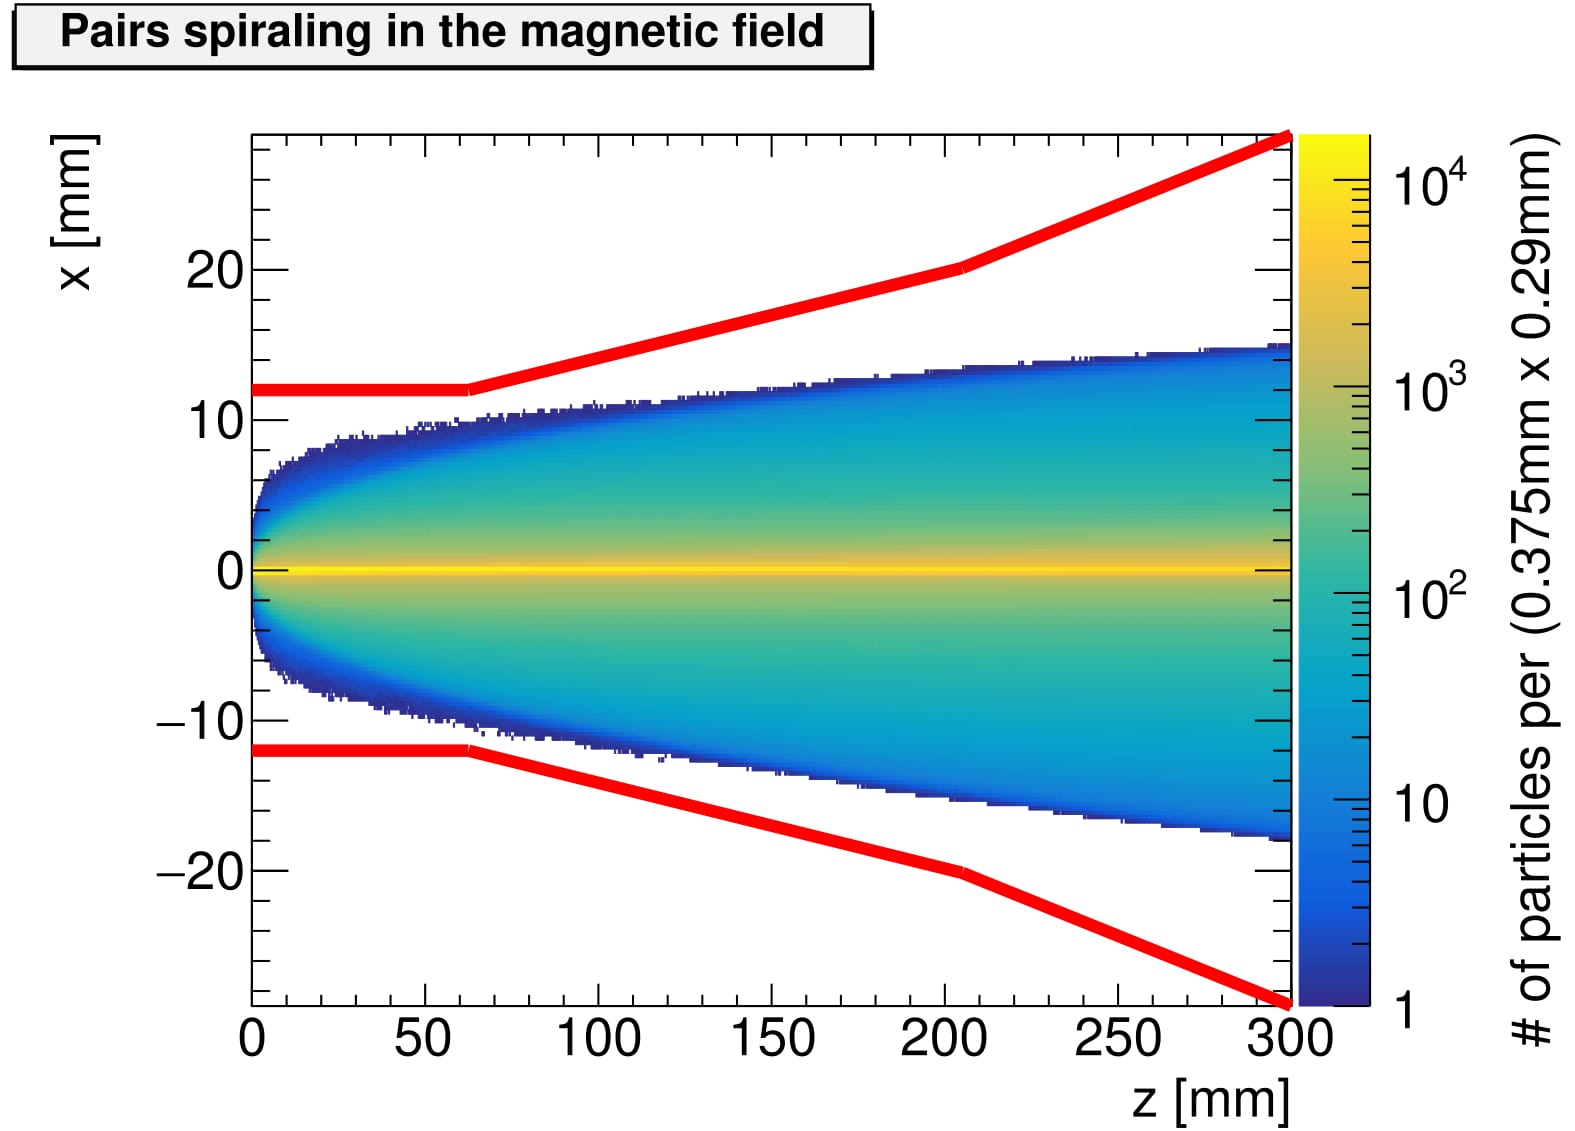
\includegraphics[width=\textwidth]{figures/Helix_tracks_xz_100bunches_250GeV_5T_DanielJeans-1.jpg}
\caption{\textit{ILC250 set (TDR)}}
\end{subfigure}
\hspace*{0.08cm}
\begin{subfigure}[t]{0.49\textwidth}
\centering
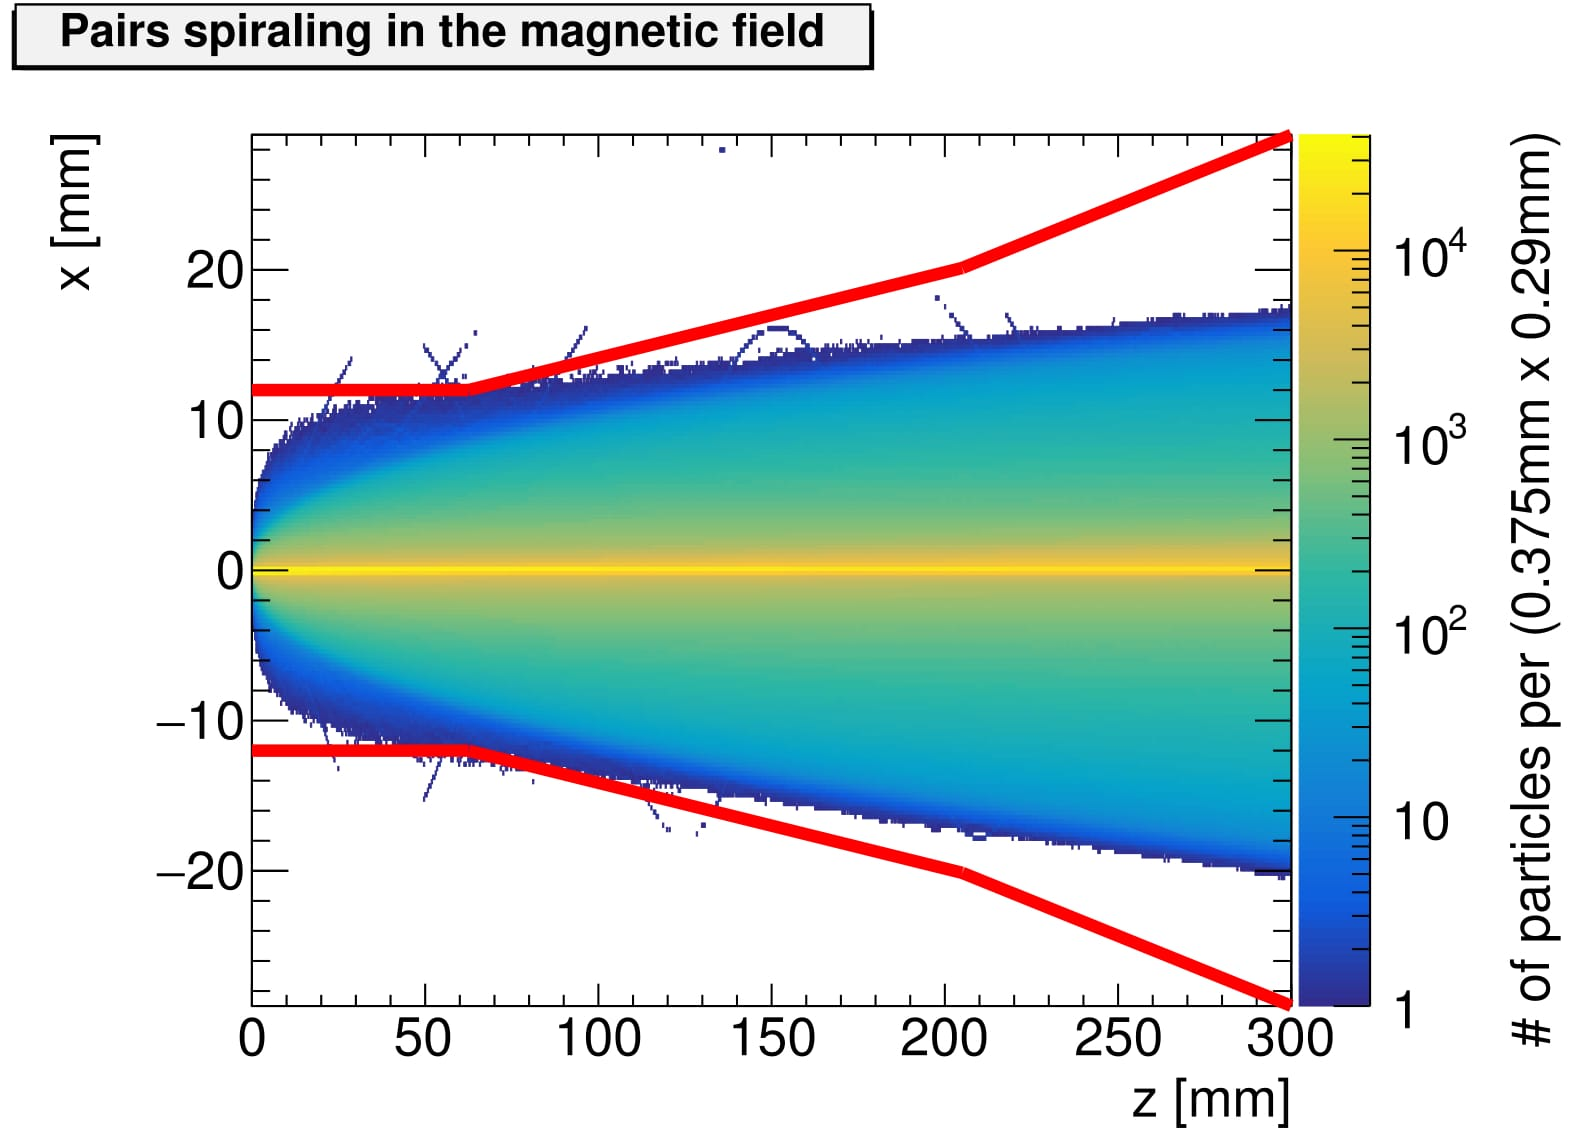
\includegraphics[width=\textwidth]{figures/Helix_tracks_xz_80bunches_250GeV_5T_Reduced_Emittance_x-1.jpg}
\caption{\textit{ILC250 set (A)}}
\end{subfigure}
\\
\begin{subfigure}[t]{0.49\textwidth}
\centering
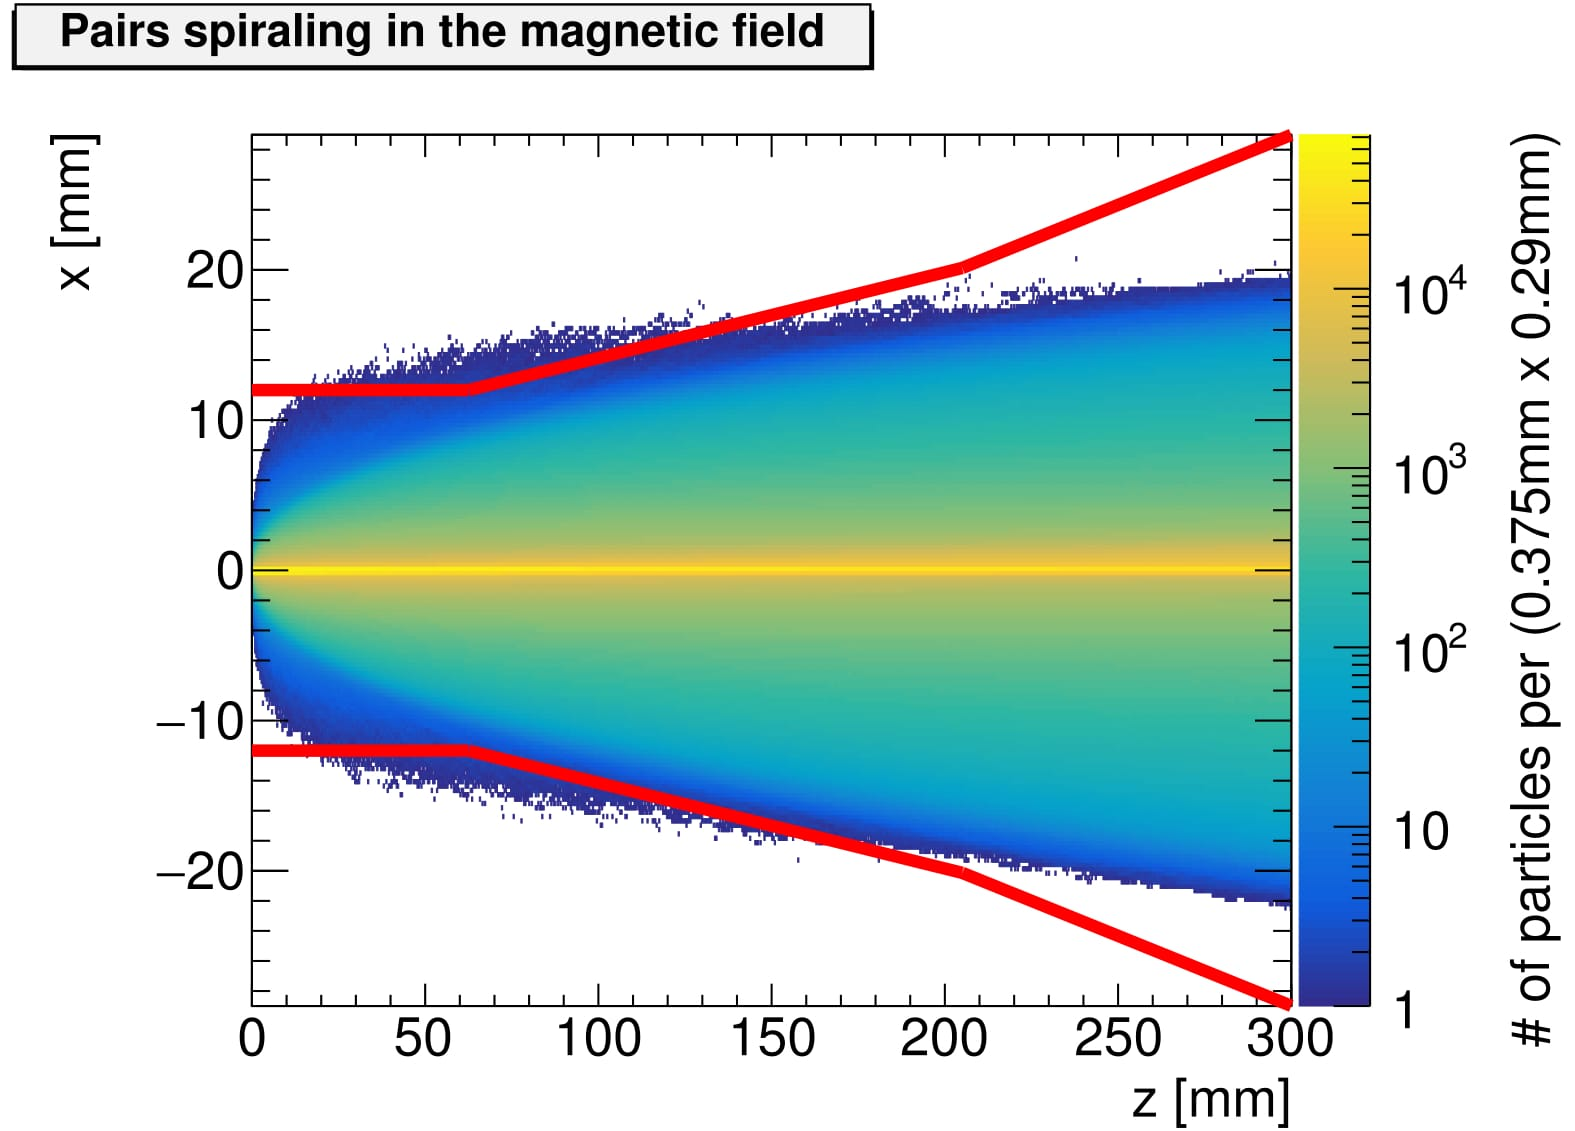
\includegraphics[width=\textwidth]{figures/Helix_tracks_xz_50bunches_250GeV_5T_Reduced_Emittance_x_Reduced_Beta_x-1.jpg}
\caption{\textit{ILC250 set (B)}}
\end{subfigure}
\hspace*{0.08cm}
\begin{subfigure}[t]{0.49\textwidth}
\centering
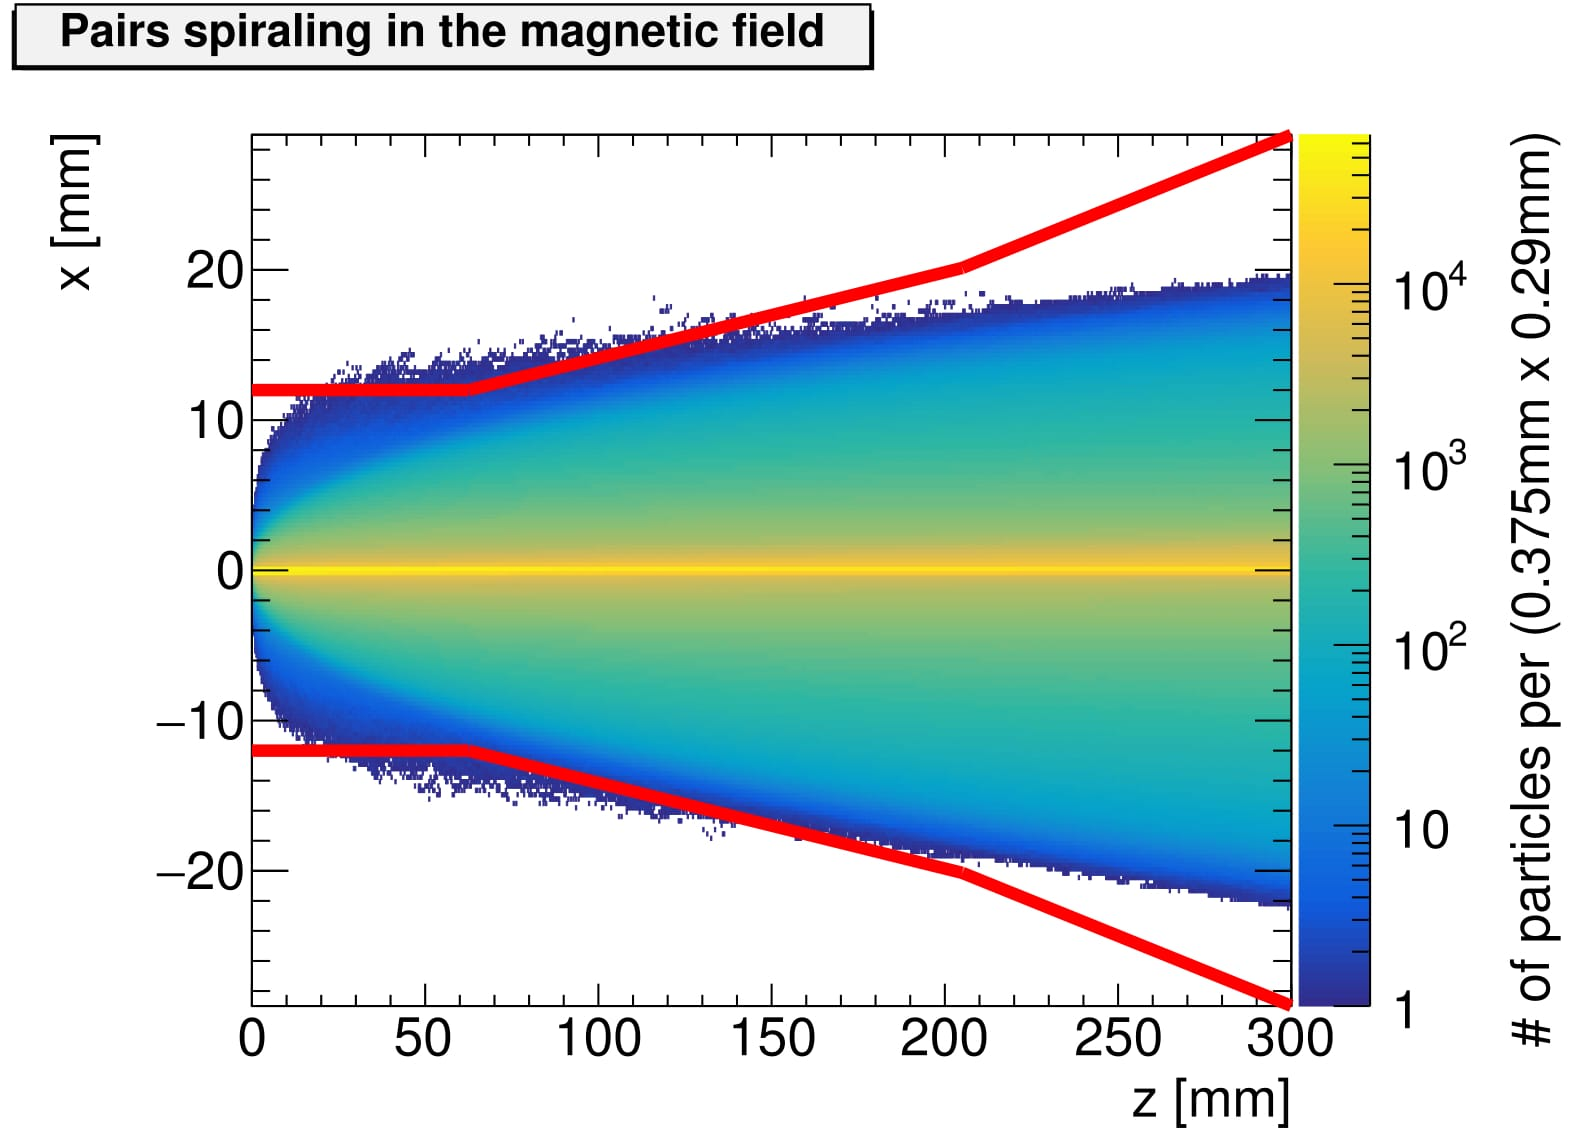
\includegraphics[width=\textwidth]{figures/Helix_tracks_xz_50bunches_250GeV_5T_Reduced_Emittance_x_Reduced_Beta_x_Increased_Beta_y-1.jpg}
\caption{\textit{ILC250 set (C)}}
\end{subfigure}
\caption{\textit{Pair background density for the different ILC250 beam parameter sets for a full bunch train (1312 bunch crossings). Although the pairs are deflected in the SiD solenoid field, the high-p\textsubscript{T} pairs reach past the beam pipe towards the inner layers of the detector. The beam pipe is represented by the red solid lines.}}
\label{fig:Envelopes}
\end{figure}

\begin{figure}
\centering
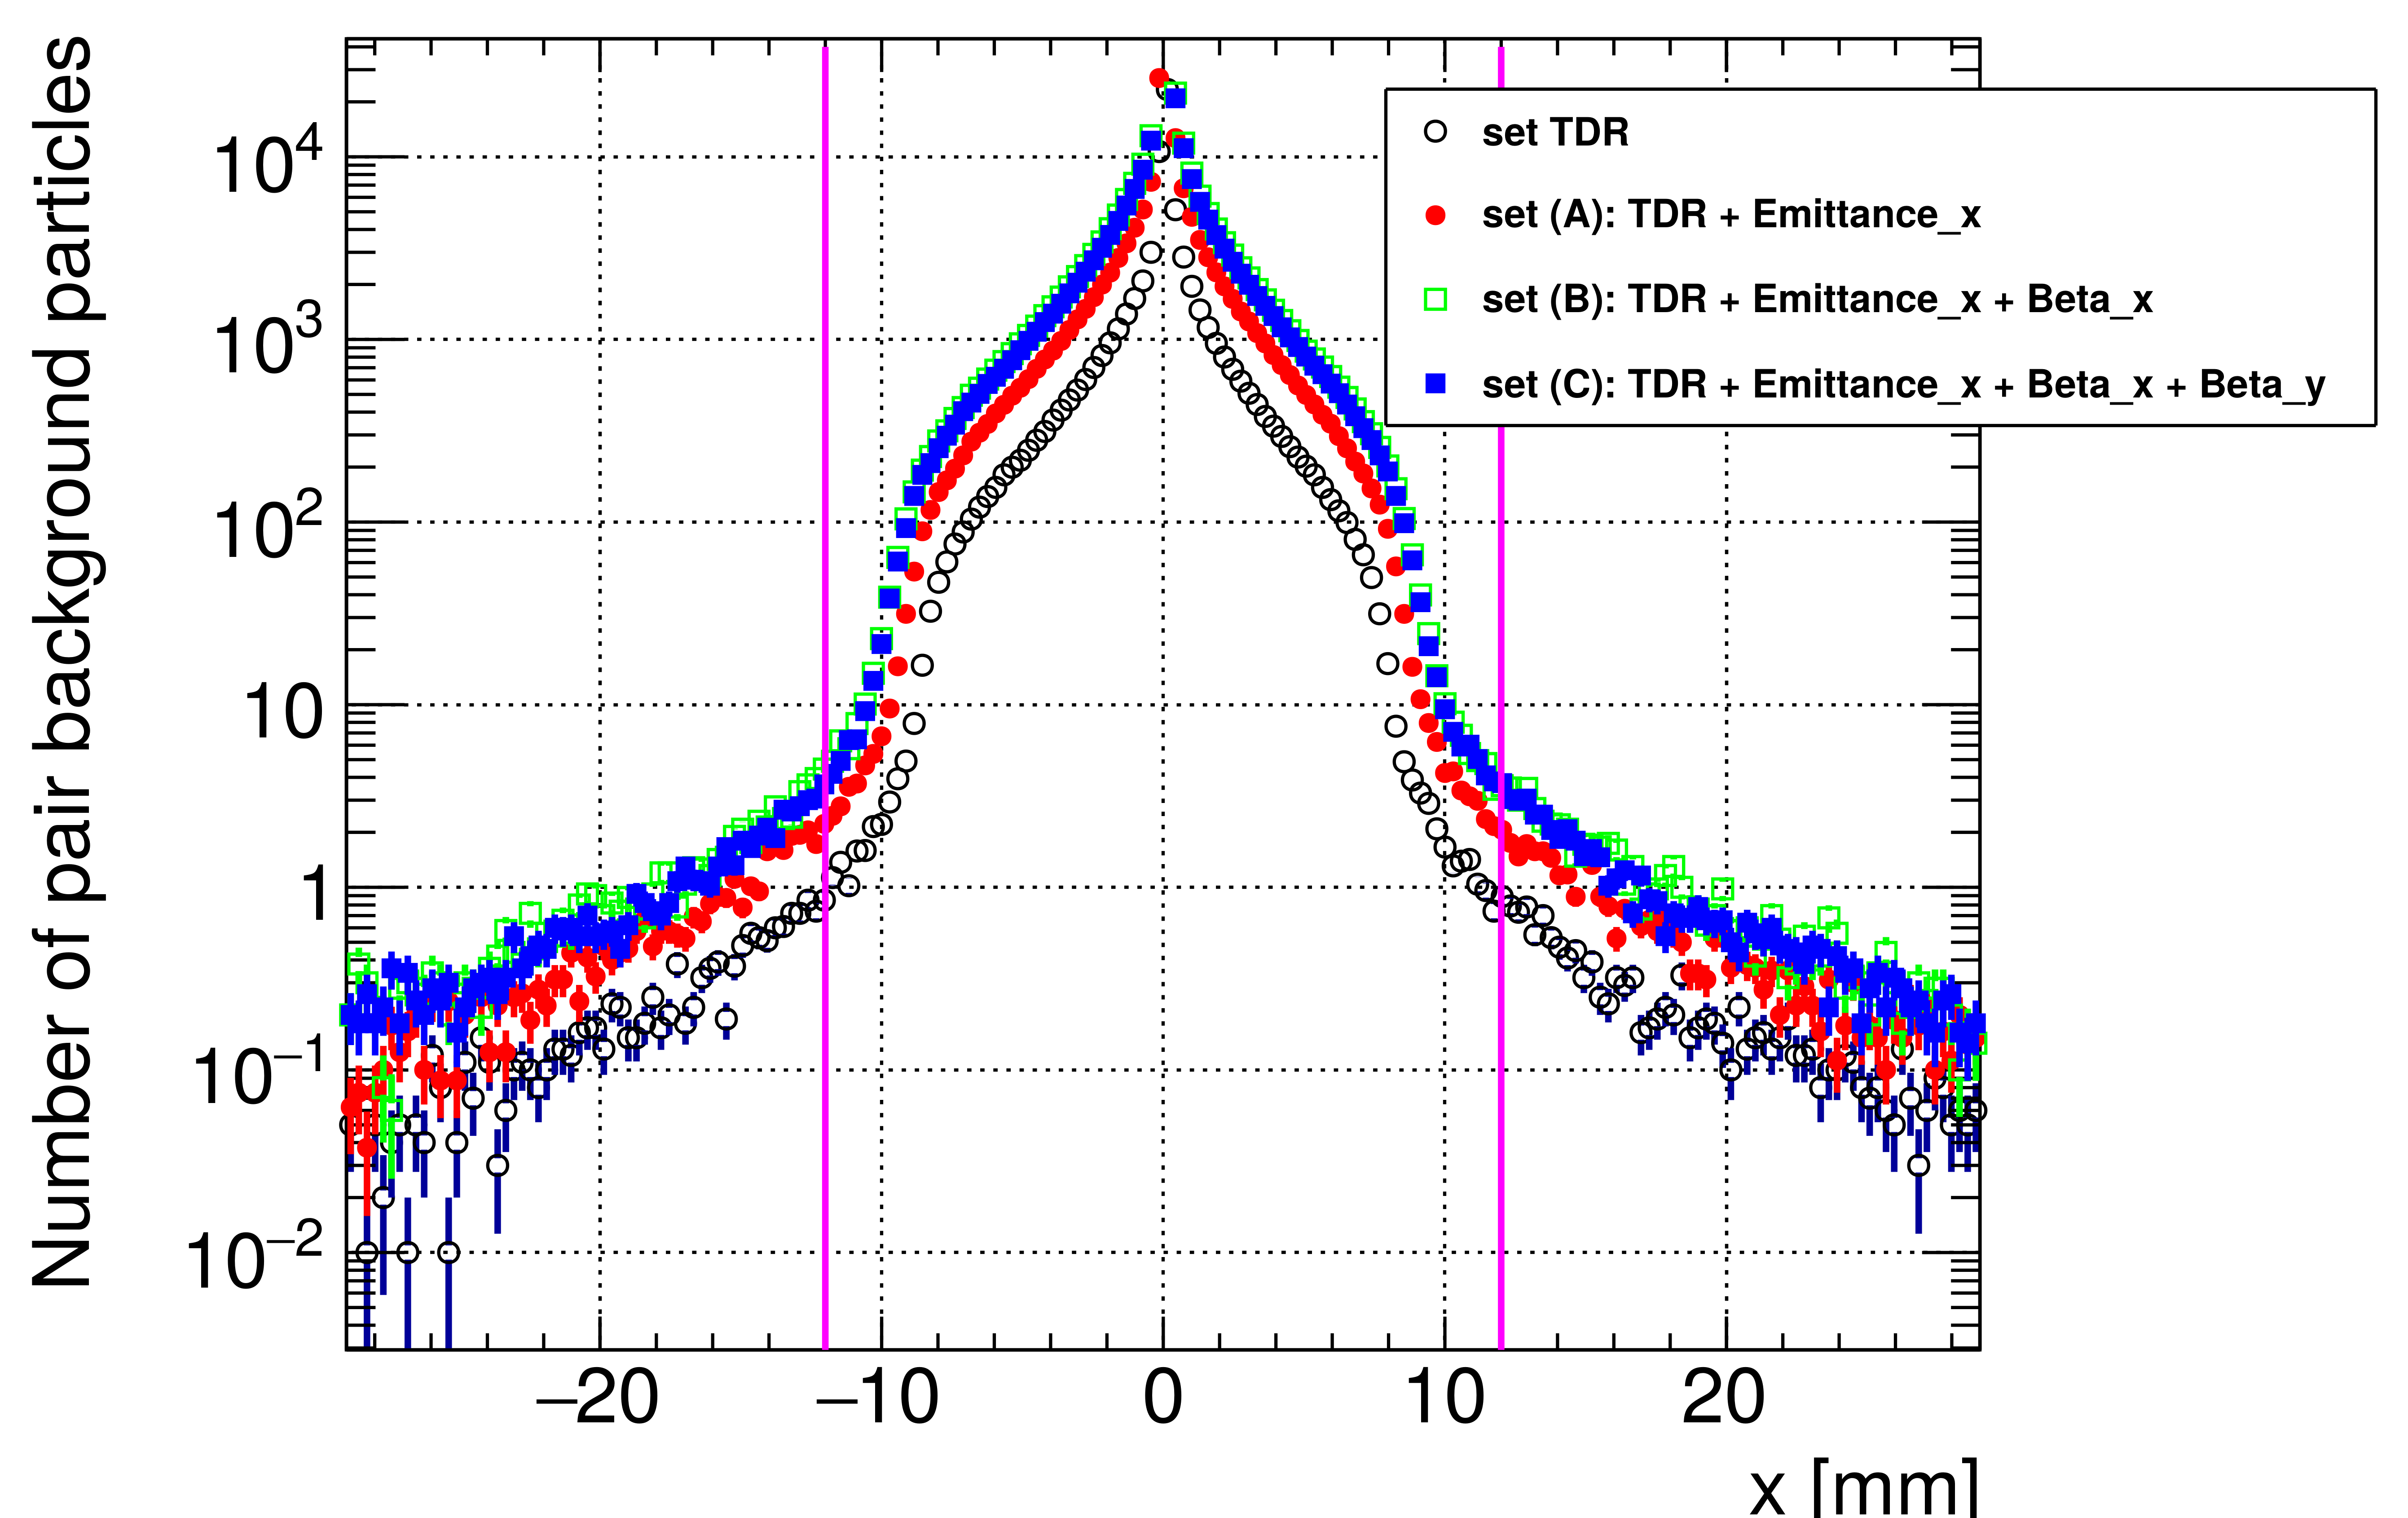
\includegraphics[width=0.78\textwidth]{figures/HelixEnvelope_Projection_Comparison_250GeV_parametersets_LEG.png}
\caption{\textit{Projection of the pair background density for a full bunch train (1312 bunch crossings), which is shown in Figure~\ref{fig:Envelopes}, along the x direction.
The projection is done for z $=$ \SI{62}{\milli\meter}, the z position of the first beam pipe kink.
At that position, the background envelopes are the largest compared to the beam pipe radius.
The beam pipe is indicated by the pink solid lines.}}
\label{fig:Projection_Envelopes}
\end{figure}
\iffalse
    The projection of the helix tracks from the pair background particles of one bunch crossing are shown in the xz- and yz-plane in Figures a) and c).
    The color scales shows how many particle tracks are in the single bins of these plots.
    To get a better grasp, Figures b) and d) show the envelopes outlining certain fractions of helix tracks.
    Therefore, the blue line represents the envelope of 99\% of all pair tracks.
    In all subfigures, the thin red lines represent the beam pipe.
    The helix tracks were calculated for a homogeneous magnetic field of \unit{5}\,{T}.
\fi
%\input{VXD_Occupancies}
%\section{Summary and conclusion}
By looking at the luminosity spectra generated for this study, the expected increase in luminosity for the new ILC250 parameter sets could be confirmed.
The background studies indicate that the new official beam parameter set (set (A)) increases the \Pep\Pem pair background density and the SiD vertex detector occupancy by only a factor of about 2-3 in comparison to the original TDR beam parameters.
Although the density of the pair background close to the interaction point rises, the normalized vertex detector occupancy for the new set is well below 10$^{-4}$.
The SiD Optimization group is confident that this can be accommodated in the design of the SiD vertex detector without a loss in precision for the physics studies.


\section*{Acknowledgments}
The author would like to thank the SiD Optimization group, as well as Daniel Jeans (KEK) for useful discussions and helpful input to the presented studies.

%\section{Appendix}


%% References with bibTeX database:

\bibliographystyle{unsrt}
%\bibliographystyle{model1-num-names} %Doesn't work well if you also cite webpages (Confluence page)
\bibliography{bibliography.bib}

\end{document}
